\section{Prototyp Testplan}
\label{sec:testabnahme}
Überprühfung der Anforderungen.
\subsection{Abnahme-Testplan}
T1. Die Türe bei der Aussensprechstelle muss nach betätigen der «Türe öffnen» Taste in der Client-App, geöffnet werden können.
\\
\\
T2. In der Client-App wird ein Videosignal von der Kamera bei der Aussensprechstelle erhalten. 
\\
\\
T3. Durch Bedienen der Client-App wird ein Audiosignal von der Aussensprechstelle erhalten und umgekehrt. 
\\
\\
T4. An der Aussensprechstelle kann man die Namen den Bewohner lesen und auswählen.  
\\
\\
T5. Die Stromversorgung der Anlage wird aus- und dann wider eingeschaltet. Die Anlage muss ohne externe Eingriff wider Starten. 
\\
\\
T6. Mithilfe von Wireshark wird den Netzwerkverkehr analysiert. Den gesamten Datenverkehr aus der Anlage ist verschlüsselt. 
\\
\\
T7. Feuchtigkeit, Temperatur und Betriebsbedingungen aus dem Datenblatt mit den Anforderungen vergleichen und überprüfen.
\\
\\  
T8. Durch eine Analyse wird die effektive Auflösung des Videosignales evaluiert. Die Auflösung muss mindestens 720p (ev. 1080p) aufweisen. 
\\
\\
T9. Sämtliche Materialkosten zusammenstellen und überprüfen. Die Kosten pro Aussensprechstelle müssen das in den Anforderungen definierten Maximum, nicht überschreiten. 
\\
\\
T10.  Mit bedeckte (Skihandschuh) und/oder nasse Hände muss man bei der Aussensprechstelle Klingeln können. 
\\
\\
T11. Bei der Aussensprechstelle ist nur der Netzwerkkabel zu finden, keine zusätzliche Speisung. 
\\
\\
T12.  Bei Klingeln und nicht öffnen der Türe, muss in der Client-App den Verpassten Besuch sichtbar sein. 
\\
\\
T13. Durch Bedienen der Client-App ist es möglich frei zu sprechen ohne, dass das Audiosignal an der Aussensprechstelle weitergeleitet wird.
\\
\\
Ergebnisse werden in einer Test‐Traceability Matrix visuell festgehalten. Jede Anforderung wird  durch  einen  Test  überprüft.  Beziehungsweise verifiziert jeder Test nur die betroffene Anforderung. Auf diesen Wege werden Überschneidungen vermeiden.
\subsection{Resultate}
Alle Tests bis auf zwei, wurden bestanden. (\seeref{fig:testmatrix})
\\
Es werden nun die Anforderungen und Tests aufgelistet, welche nicht bestanden wurden.
\subsubsection{Test 12: Verpasste Besuche sind in der Client-App ersichtlich}
Bei Test 12 wird eine Wunschanforderung geprüft: \textit{(W13. Verpasste Besuche sollten aufgezeichnet werden und in der Client App in Form von einem Foto und Notifikation sichtbar sein)}. Diese Funktionalität wurde aus Zeitgründen nicht vollständig implementiert. Die Anforderung wurde daher nur teilweise erfüllt. Wenn jemanden an der Türe klingelt, wird auf den mobilen Gerät eine Benachrichtigung angezeigt. Diese bleibt solange sichtbar bis der Benutzer Diese gelesen hat und löscht. Demzufolge sind verpasste Besuche trotzdem ersichtlich, auch wenn sie im Web-App nicht erscheinen.
\\
Da es sich um eine Webbapplikation handelt, kann diese Funktionalität ohne grosses Know-How von anderen beteiligten Technologien nachträglich implementiert werden.

\subsubsection{Test 8: Die Auflösung des Videosignales wird evaluiert}
Test 8 prüft zwei Anforderungen. Es handelt sich um die zwei folgenden:
\begin{itemize}
	\item A9: Die Kamera für das Videosignal muss eine Auflösung von mind. 1280x720 Pixel aufweisen. 
	\item W2: Die Kamera für das Videosignal muss eine Auflösung von 1920x1080 Pixel aufweisen. 
\end{itemize}
Im Nachhinein ist uns klar geworden, dass diese zwei Anforderungen und ihre dazugehörigen Tests besser definiert werden könnten. 
\\
\\
Der Test lautet: \textit{ Durch eine Analyse wird die effektive Auflösung des Videosignales evaluiert. Die Auflösung muss mindestens 720p (oder 1080p) aufweisen.}
\\
Die Eingesetzte Kamera weist effektiv eine Auflösung von 1920x1080 Pixel. Das Problem hier liegt bei der Digitalisierung des Videosignales. Währen der Fachmodul-Phase wurde die Komplexität der Video-Encoding unterschätzt.
\\
Demzufolge besitzt nun unser System die Hardware um diese Anforderungen zu erfüllen aber nicht die Rechenkapazität.
\\
Wie in der \cref{sec:AussensprechstelleWebapplikation} bereits diskutiert, wäre hier eine bessere CPU eine mögliche Lösung.
\begin{figure}[htb!]
	\begin{center}
		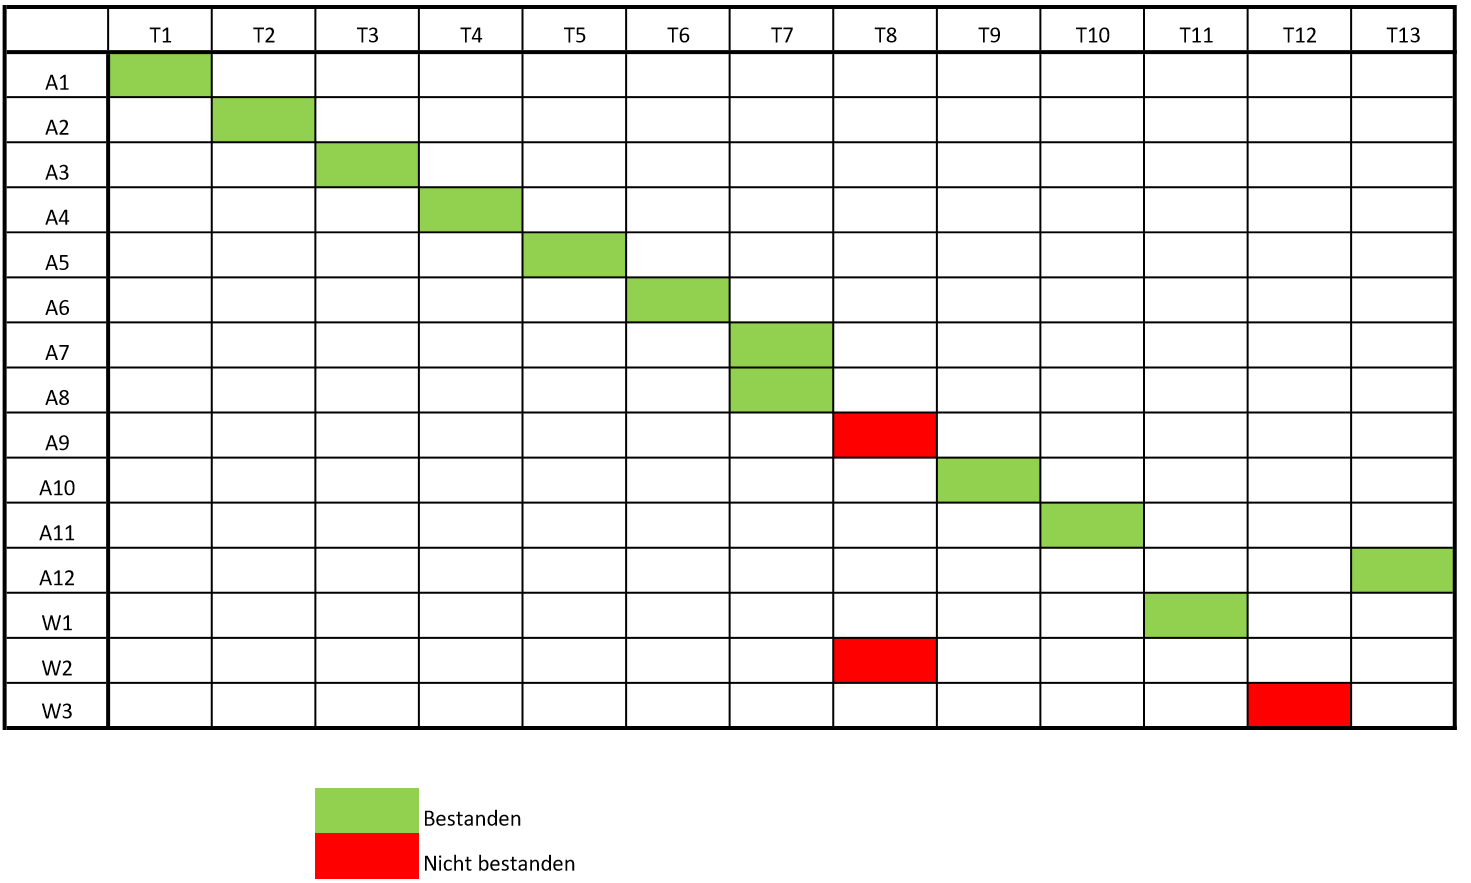
\includegraphics[width=1\textwidth]{testmatrix}
		\caption[Test-Traceability Matrix]{Test Traceability Matrix}
		\label{fig:testmatrix}
	\end{center}
\end{figure}

\newpage